\lhead[\thepage]{ANEXO 1.  Summary}
\chead[]{}
\rhead[WepSIM: Simulador de un procesador elemental con unidad de control microprogramada\leftmark]{\thepage}
\renewcommand{\headrulewidth}{0.5pt}

\lfoot[]{}
\cfoot[]{}
\rfoot[]{}
\renewcommand{\footrulewidth}{0pt}




\chapter*{Anexo 1: Summary}
\addcontentsline{toc}{chapter}{Anexo 1: Summary}
\markboth{}{APPENDIX A}

\section*{Introduction}

Teaching the architecture of a computer is a basic and fundamental part of the training of computer science students, through which students achieve a low-level vision and understanding of behavior in a computer. In order to get students to understand and correctly understand the theoretical foundations, it is necessary to use practical classes, where the student can be able to interact with a computer of architecture similar or similar to that explained in theory and also manage to extrapolate the theoretical foundations To actual behavior.

One of the main problems when designing these practical classes is to obtain the necessary means so that the students can use a computer similar to that seen in the theoretical classes, due to the cost of having a sufficient number of computers for the Number of students who must make use of them and their maintenance, the limitation of mobility when doing the practices due to the physical need of the computer, etc. To avoid these problems, simulators and emulators are currently used to provide the necessary functions for the practical classes, avoiding the problems discussed above.

An emulator is a software that imitates the behavior of a computer so that programs designed for a particular architecture can be executed in a different one. On the other hand, a simulator is a software that tries to reproduce the behavior of a computer, but with a lower level of realism, since the emulator is in charge of accurately modeling the device so that the programs executed on it work as if Were being executed in the original device.

There are different simulators that can be used to work with the main aspects that are treated in the subjects of Structure and Architecture of Computers: assembler, cache, etc. Most of these simulators focus on a specific type of simulation, which implies a loss of the vision of the set when needing the use of different simulators. Therefore it is much better to always have a centralized vision of any service, being more favorable the use of a tool that combines the maximum possible functionalities.

There is another problem not least: most of the simulators are designed for PC. One of the goals we put forward with WepSIM is that it could be used in smartphones or tablets, to offer the student greater flexibility in its use.

In addition to having a portable simulator to different platforms, the simulator must be as self-contained as possible, so that it integrates the main help for its use (not as a separate document that serves as a user manual to be printed) allowing the user to do A full use of the application without the need to get out of it.

Therefore, we have considered how to offer a simulator that is simple and modular, and that allows to integrate the teaching of the microprogramming with the programming in assembler. In particular, it can be used to microprogram an instruction set and see the basic operation of a processor, and to create assembler programs based on the assembler defined by the above microcode. This is of great help, for example, for the programming of systems since it is possible to see how the software interacts in assembler with the hardware in the treatment of interruptions. The idea is to offer a simulator that offers a global vision of what happens in hardware and software, also avoiding the extra time involved in learning different tools.


\section*{Objectives}

The main objective of this project is to develop a simulator, which unlike the existing ones, can fully simulate the behavior of an elementary processor allowing to check the state of the components in each clock cycle, so that it helps the students To understand and assimilate in a simple and visual way the operation of a processor. The secondary objectives, derived from the main objective, are:

\begin{itemize}

\item \textbf{O1:} Simulate the execution of the set of instructions specified in a computer called WepSIM from the point of view of microprogramming and programming in assembler.

\item \textbf{O2:} Allow specification of different sets of instructions.

\item \textbf{O3:} Allow unified microprogramming in a computer and programming in assembly language.


\item \textbf{O4:} Allow the user to display in each clock cycle the status and behavior of the simulated computer.

\end{itemize}

\section*{WepSIM Elemental Processor}

WepSIM is an elementary processor with microprogrammed control unit designed by the staff of the research group ARCOS of the University Carlos III of Madrid for teaching in the subject Computer Structure.

In the figure \ref{fig:wepsimCPU_figure_summary}, the structure of the WepSIM Elemental Processor is shown. WepSIM consists of a memory module, a keyboard device, a display device and a generic I/O device that can be used to work with interrupts.

\begin{figure}[htbp]
 	\centering
 	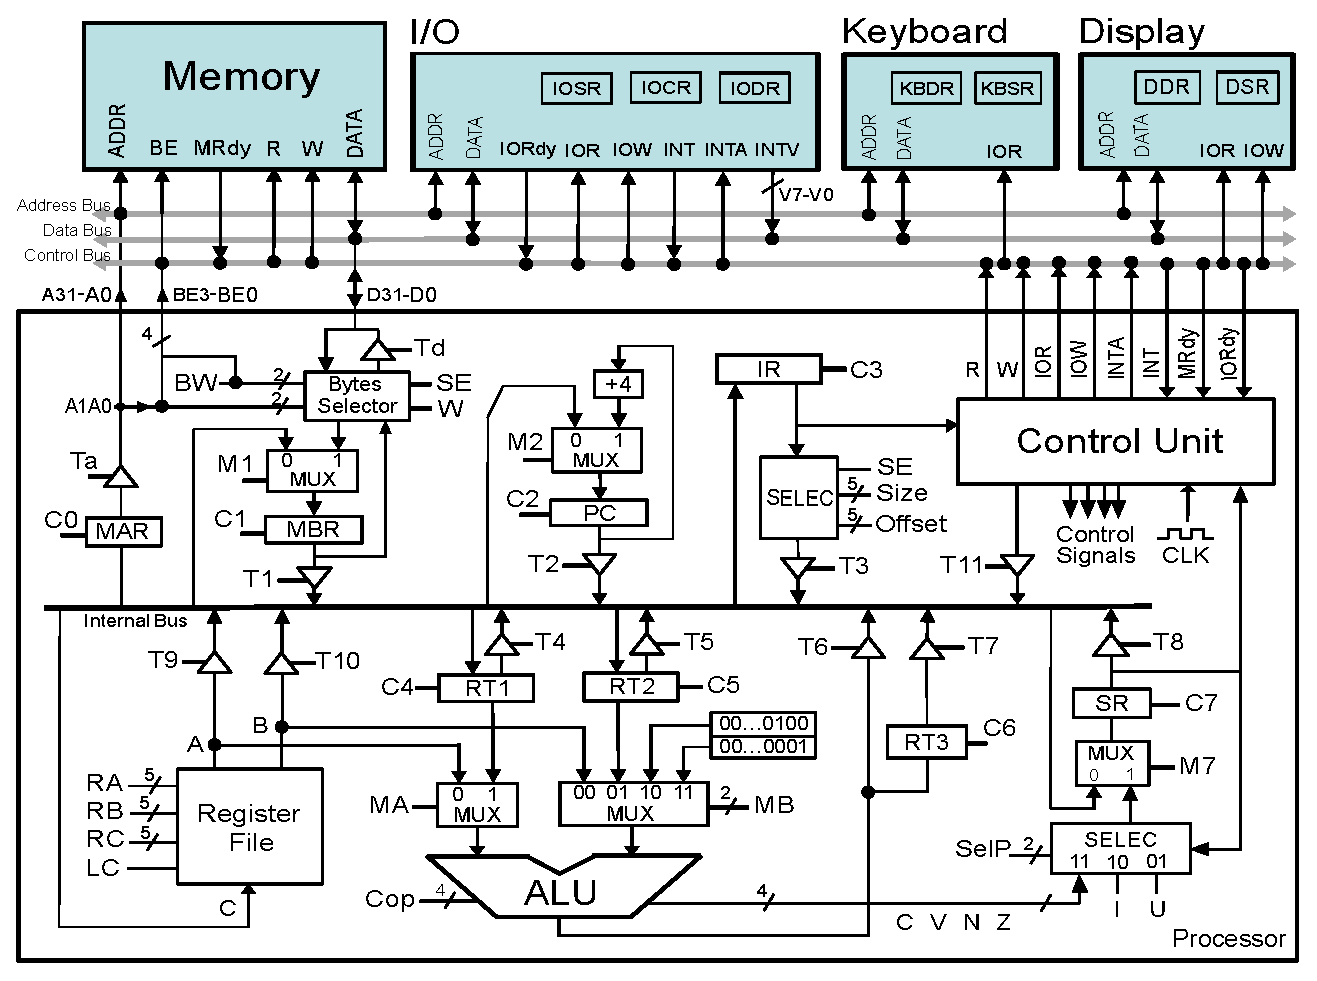
\includegraphics[width=11cm]{figures/processor6}
 	\caption{CPU Architecture WepSIM .}
	\label{fig:wepsimCPU_figure_summary}
\end{figure}

\begin{figure}[htbp]
 	\centering
 	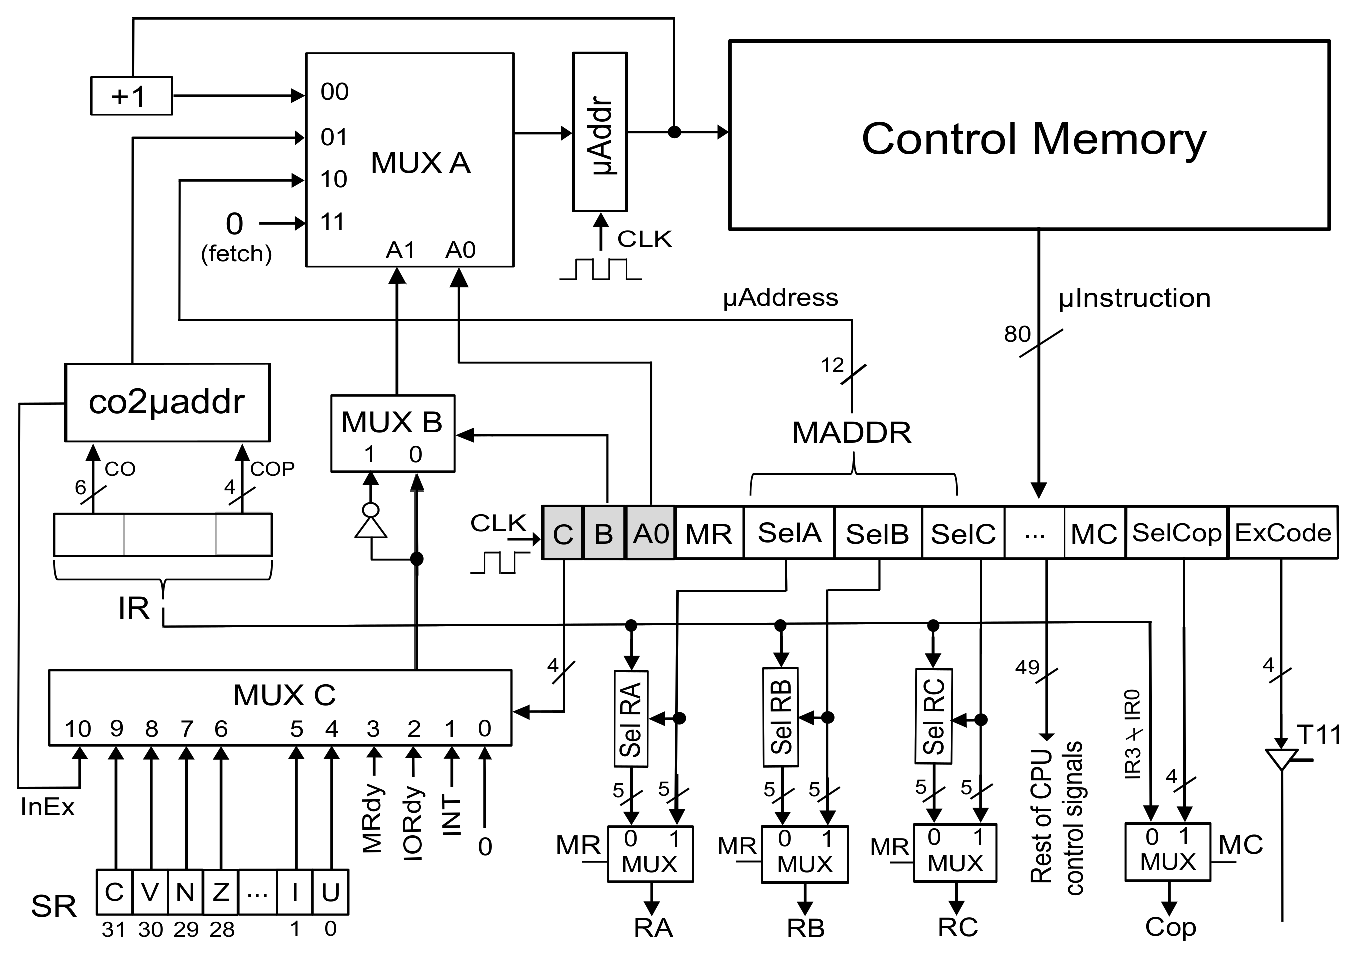
\includegraphics[width=11cm]{figures/controlunit6}
 	\caption{Arquitectura unidad de control WepSIM.}
	\label{fig:wepsimCU_figure_summary}
\end{figure}


WepSIM is a 32bit processor that addresses memory by bytes, which has a bank of 32 registers and two additional registers (RT1 and RT2) that are not visible to the assembler programmer but allow temporary storage of data for the carrying out of intermediate operations. From the registers, it is possible to send the values to operate in an ALU that hasta the 15 most most common arithmetic-logic operations.  The PC registry has its own operator adding four, so it is not necessary to make use of the ALU for this operation. The result of the operations performed in the ALU can be stored in a temporary register (RT3) that is also invisible to the assembler programmer, or sent directly to the internal bus through the corresponding tristate.


The status register (SR) can be updated with the resulting flags of the last operation of the alu (O, N and Z). To do this, SELEC/SelP represents a circuit block that allows indicating which part of the state register (SR) must be updated. To the right of SELEC/SelP the bits of the SR status register enter (Input = ONZIU) and SelP allows to select which group of these bits will be updated in the status register: bits O, N and Z with the values coming of the ALU, the bit I with the indicated value or the bit U with the indicated value for the same.

The instruction register (IR) is associated with a selector module (higher level circuit than a multiplexer, etc.) which allows to select a segment of the binary value stored in the instruction register that will pass to T3.

In particular, the position (Offset, where 0 represents the least significant bit of the IR register) and the number of bits (Size) to be taken from that initial position is indicated, and if it is desired to make sign extension (SE ) Before passing the value to the T3 input.

The MAR and MBR registers are used to store the address and content associated with this address in read/write operations with memory. The memory is designed for synchronous or asynchronous operation. It currently works synchronously, but has the MRdy signal for future work asynchronously. The selection circuit allows you to indicate which portion of the memory word is the desired one (one byte, two bytes, or a complete four-byte word).

There are also three I / O devices: a keyboard, a display and a generic device that can be configured to generate various types of interrupts.

Finally, the Control Unit generates the control signals for each clock cycle. The Figure \ref{fig:wepsimCU_figure_summary} Shows the Control Unit in more detail. It is a microprogrammed control unit with implicit sequencing. The control signals for the current clock cycle are stored in the micro-instruction register (the one with the fields A0, B, C, SelA, etc.). The contents of this record come from the control memory, specifically from the content in the position to which the micro-address register points. The micro-address stored in this register can be modified using the ``MUX '' multiplexer. There are four options: the current micro-address plus one, a micro-address indicated in the micro-instruction itself (which overlaps with SelA, SelB and partially with SelE), the first micro-address associated with the operation code field of the instruction of the IR register, and finally the value zero, which is the address of the control memory where the microprogram corresponding to the fetch is stored. The micro address can be selected conditionally by using the ``MUX C '' multiplexer that allows to select the status register bits (SR) or values of the I/O control signals. 

The SelRA, SelRB and SelRE selector circuits are used to generate the values corresponding to the selector signals of the register bank RA, RB and RE. These selectors take as input the 32 bits of the instruction register (IR) on one side and the field SelA, SelB and SelE on the other, so that they take SelX as the displacement within the instruction register (from 0 to 32) from where Take the next 5 bits corresponding to the RA, RB or RE signals. They thus allow to select 5 consecutive bits of the 32 bits of the instruction register.

The MR multiplexer is used to indicate whether the RA, RB and RE signals are literally the values stored in SelA, SelB and SelE (MR = 1) or if SelA, SelB and SelE indicate the offset within the instruction where the values to be used for RA, RB and RE. The latter allows the instruction to indicate the registers to be used as operands in the register bank, instead of indicating them from the micro-instruction.

For the Cop signal (operation code in the ALU), the MC signal can be used to take the SelCop value of the micro-instruction (MC = 1) or the 4 least significant bits of the instruction register (MC = 0), ie IR3 -IR 0.

\section*{Simulator design}

In order for the teachers of the Computer Structure subject to use a tool that helps to explain the theoretical concepts of the subject, and students can use it to understand these concepts and to carry out the subject's practices later, Proposes the design and implementation of a web tool that realistically simulates an elementary processor with a microprogrammable control unit.

This simulator will be developed as a web tool due to the portability it provides, since it can be executed on a large number of different devices regardless of the operating system you use, since you only need a web browser for its correct operation. In this way, teachers and students will be able to use the tool without depending on their installation in the device to be used, even if students can practice on mobile devices.

To achieve this portability, the simulator has been developed in HTML5 (HTML + JavaScript + CSS) making it possible to run on any platform (smartphones, tablet, PC, etc.) that can run Microsoft Edge, Mozilla Firefox, Google Chrome or Safari. In addition, the tool depends on the following frameworks / libraries: JQuery, JQueryUI, JQuery Mobile, Knockout and BootStrap.

Therefore, the chosen solution is able to unify in a single tool all the functionalities required for the teaching of Structure of computers with a high level of detail, with high availability by facilitating its as a web tool, and with a great portability since Can be executed on a large number of different devices, always looking for a solution without the need for a server.

\subsection*{Simulator Architecture}

The architecture of the solution presented in this work consists of three main elements:

\begin{itemize}
\item \textbf{Hardware model:} allows you to define the hardware to use.
\item \textbf{Software model:} allows to define the set of instructions to use.
\item \textbf{Simulation kernel:} simulates hardware operation by running microcode / machine language previously defined.
\end{itemize}

The hardware model allows to define the typical elements of a computer (main memory, processor, etc.) in a modular way. The way in which these elements are defined balances two opposing objectives: it is sufficiently complete to imitate the main aspects of reality, but it is sufficiently minimal to facilitate its use. Above all, it is intended to be a didactic tool.

The software model allows defining the microcode and assembler based on this microcode as intuitively as possible. The assembler to use is given by a set of instructions that can be defined by the user and tries to be flexible enough to be able to define different types and sets of instructions, such as MIPS or ARM.

The third element of the proposed architecture is a kernel that takes as input the described hardware model and the working software model, and is responsible for showing the operation of the hardware with the given software.

\begin{figure}[htbp]
 	\centering
 	\includegraphics[width=14cm]{figures/architecture_diagram}
 	\caption{WepSIM Architecture.}
	\label{fig:architecture_diagram_summary}
\end{figure}

The Figure \ref{fig:architecture_diagram_summary} summarizes the architecture of WepSIM. The starting point is the hardware model that describes the processor to be simulated. This includes the processor, memory, and some I / O devices: keyboard, display, and a single I / O device that generates interrupts. The hardware model describes the overall state of the processor. From the processor's overall state, the simulation kernel updates the state in each clock cycle.

The simulated control unit stores the control signals of each cycle in a control memory. The control memory has all the microprograms for the instructions with which the processor works, and the fetch to read the memory instruction and to decode it.

The microcode (the contents of the control memory) together with the format of each instruction (fields of the instruction and its length) is described in a text file. The software model reads this file, translates it to binary and loads it into the processor. The definition of the assembler language to be used is described together with the microcode, and the software model allows to translate programs written in said assembler to binary.


The simulation kernel asks the subsystem of the software model for the defined microcode, the description of the instruction format and the contents of the main memory. The binaries are loaded into the elements of the hardware model, and then the simulation kernel updates the global state in each clock cycle.

WepSIM has a simulation controller that is responsible for updating the clock cycle and displaying the global status. The simulation interface subsystem updates the user interface. When the user uses the user interface to request an operation, the simulation interface subsystem moves the request to the simulation controller. In this way, a basic Model-View-Controller (MVC) is used for the WepSIM architecture.

\section*{Conclusions and future work}

This section presents the conclusions of the paper, reviews the objectives set out at the beginning of this document, and includes some personal conclusions. In addition, we discuss the main contributions of our work, also indicating the publications resulting from this work. Finally, future work is discussed.

\section*{Conclusions}

In this work we have described the design of WepSIM, a simulator of an elementary processor with microprogrammed control unit. This work presents a new simulator that is intuitive, portable and extensible, serving as a teaching complement for teaching in Computer Structure. This simulator allows you to define different sets of instructions and to execute and debug source code using the defined set of instructions. It also allows to define the behavior of the processor by microprogramming.

WepSIM allows students to understand the operation of an elementary processor in a simple way, can be used from a mobile device or a computer with a modern Web browser without the need to be installed. In this way, students can interact with the simulator by learning and understanding the operation of the WepSIM elementary processor, including the mechanisms of interaction with the system software and integrating in the same tool both the microprogramming and the programming in assembler.

The main objective of this project was to develop a simulator, which, in contrast to existing ones, could completely simulate the behavior of an elementary processor, allowing to check the state of the components in each clock cycle, so that students Understand and assimilate in a simple and visual way the operation of a processor. We have also met all the other objectives presented in the introduction of the document:

\begin{itemize}

\item \textbf{O1}, A tool has been designed that simulates the execution of the instruction set specified in a computer called WepSIM, from the point of view of microprogramming and assembly programming.

\item \textbf{O2}, The tool allows the specification of different instructions.

\item \textbf{O3}, The tool unifies the microprogramming of a computer and programming in assembler language.

\item \textbf{O4}, The tool allows the user to display in each clock cycle the state and behavior of the simulated computer.

\end{itemize}

On a personal level, this work has helped me to enter the world of scientific research. I have been able to apply a great deal of the knowledge acquired throughout the degree. In addition, I have learned important techniques of hardware modeling, compilation and simulation, which have a great utility and complexity and have served me to deepen even more in the knowledge acquired in the degree. For all this, it is very satisfying to see the final result obtained, since I have managed to overcome all the problems that have arisen throughout the project.

\subsection*{Contributions}

The project carried out during this Work End of Degree fits with many of the subjects studied in the Degree in Computer Engineering of the Carlos III University of Madrid, highlighting the following topics in particular:

\begin{itemize}

\item \textbf{Computer technology} (Compulsory subject, First course) Where the hardware components and binary logic are introduced.

\item \textbf{Computer structure} (Compulsory subject, Second course) Where the bases of the structure and operation of a computer are introduced.

\item \textbf{Formal languages and Automata theory} (Compulsory subject, Second course) Where the bases are introduced about the formal languages and grammars.

\item \textbf{Operating systems} (Compulsory subject, Second course) Where the bases of the operation of the operating system are introduced.

\item \textbf{Computer architecture} (Compulsory subject, Third course) Where the bases of the architecture of a computer are introduced.

\item \textbf{Operating systems design} (Compulsory subject, Third course) Where the bases of the design of the different modules of an operating system are introduced.

\item \textbf{Software development projects management} (Compulsory subject, Third course) Where the bases for the management and management of a software development project are introduced.

\end{itemize}

\subsection*{Publications}

This bachelor thesis has allowed to make an important contribution to the field of teaching in Structure and Computer Architecture. In addition, the following scientific articles have been published:

\begin{itemize}

\item \textbf{A. Calderón, F. García-Carballeira, and J. Prieto}, “WepSIM: Simulador modular e interactivo de un procesador elemental para facilitar una visión integrada de la microprogramación y la programación en ensamblador”, \textit{Enseñanza y aprendizaje de ingeniería de computadores}, vol. 6, 35-53,2016. \cite{mateos2016wepsim}

\item \textbf{J. Prieto, A. Calderón, F. García-Carballeira, and S. Alonso-Monsalve}, “WepSIM: simulador integrado de microprogramación y programación en ensamblador”, \textit{Jornadas sarteco 2016}. \cite{arcos2032}

\end{itemize}
d
In addition, at the time of delivery of this document, also another item sent waiting for its acceptance.

\vspace{1cm}

\section*{Future works}

Currently, there are several lines of future work in which we are working.

\begin{itemize}

\item Regarding improvements in the hardware model:

\begin{itemize}

\item[1.] Introduce more hardware elements, such as a cache, in order to expand the contents of the subject included in the tool.

\item[2.] Introduce a hardware model based on pipeline, allowing the use of the tool in those subjects that use this architecture model.

\end{itemize}

\item Regarding improvements in the software model:

\begin{itemize}

\item[3.] Add semantic revision of the code, allowing to identify and notify the programming errors to the user.

\item[4.] Add new sets of instructions to the tool such as the ARM assembler, allowing the use of different languages in the tool.

\item[5.] Study the MIPS / ARM assembler generated with GCC / Clang so that it can be used directly in WepSIM.

\end{itemize}

\item Regarding improvements in the tool:

\begin{itemize}

\item[6.] Add an automatic correction module of practices to the tool, so that students can practice with it and check the validity of their exercises.

\item[7.] Migrate the tool as a mobile application using the Apache Cordova plugin, so that the tool is not linked to use by web browser.

\end{itemize}

\end{itemize}

